\documentclass[tikz,border=3mm]{standalone}
\usepackage[T1]{fontenc}
\usepackage{lmodern,amsmath,amssymb}
\usetikzlibrary{arrows.meta,calc,positioning,fit,backgrounds}
\definecolor{accent}{RGB}{36,91,158}
\definecolor{soft}{RGB}{225,237,248}
\definecolor{muted}{RGB}{122,134,145}
\definecolor{warm}{RGB}{250,242,220}
\tikzset{every node/.style={font=\sffamily\small},
vertex/.style={circle,draw=black!80,fill=white,minimum size=7.5mm,inner sep=1pt},
edge/.style={draw=accent!55,line width=.65pt},
highlight/.style={draw=accent,line width=1.7pt},
box/.style={draw=accent!70,rounded corners=2pt,fill=soft!45,align=center,inner sep=6pt},
heading/.style={font=\sffamily\bfseries\normalsize,align=center},
map/.style={-{Stealth[length=2mm]},line width=.8pt},
}
\hyphenpenalty=10000\exhyphenpenalty=10000
\begin{document}
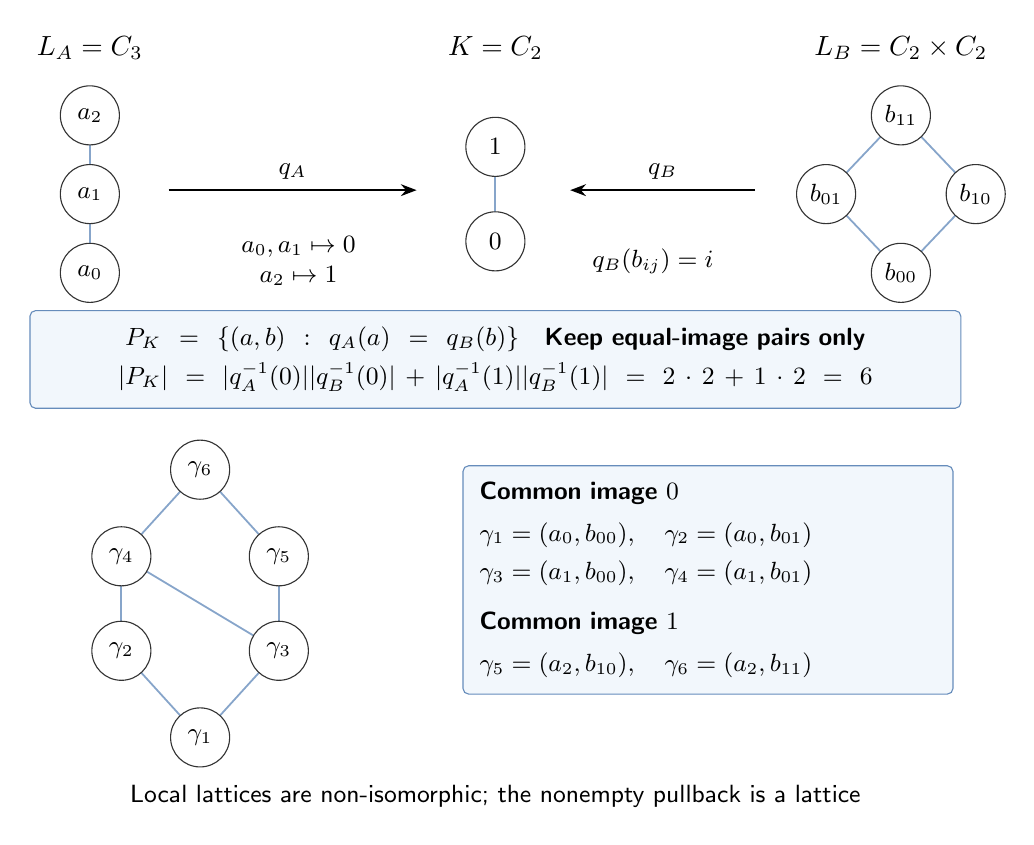
\begin{tikzpicture}[x=1cm,y=1cm]
\node[heading] at (0,6.45) {$L_A=C_3$};
\coordinate (a0p) at (0,3.6);\coordinate (a1p) at (0,4.6);\coordinate (a2p) at (0,5.6);
\draw[edge] (a0p)--(a1p)--(a2p);
\node[vertex] at (a0p) {$a_0$};\node[vertex] at (a1p) {$a_1$};\node[vertex] at (a2p) {$a_2$};
\node[heading] at (5.15,6.45) {$K=C_2$};
\draw[edge] (5.15,4)--(5.15,5.2);
\node[vertex] at (5.15,4) {$0$};\node[vertex] at (5.15,5.2) {$1$};
\draw[map] (1,4.65)--node[above]{$q_A$}(4.15,4.65);
\node[align=center] at (2.65,3.75) {$a_0,a_1\mapsto0$\\$a_2\mapsto1$};
\node[heading] at (10.3,6.45) {$L_B=C_2\times C_2$};
\coordinate (d00p) at (10.3,3.6);\coordinate (d01p) at (9.35,4.6);
\coordinate (d10p) at (11.25,4.6);\coordinate (d11p) at (10.3,5.6);
\draw[edge] (d00p)--(d01p)--(d11p)--(d10p)--cycle;
\node[vertex] at (d00p) {$b_{00}$};\node[vertex] at (d01p) {$b_{01}$};
\node[vertex] at (d10p) {$b_{10}$};\node[vertex] at (d11p) {$b_{11}$};
\draw[map] (8.45,4.65)--node[above]{$q_B$}(6.1,4.65);
\node[align=center] at (7.15,3.75) {$q_B(b_{ij})=i$};
\node[box,text width=11.4cm] at (5.15,2.50) {$P_K=\{(a,b):q_A(a)=q_B(b)\}$\quad\textbf{Keep equal-image pairs only}\\[3pt]
$|P_K|=|q_A^{-1}(0)||q_B^{-1}(0)|+|q_A^{-1}(1)||q_B^{-1}(1)|=2\cdot2+1\cdot2=6$};
\coordinate (g1p) at (1.4,-2.3);
\coordinate (g2p) at (0.4,-1.2);
\coordinate (g3p) at (2.4,-1.2);
\coordinate (g4p) at (0.4,0);
\coordinate (g5p) at (2.4,0);
\coordinate (g6p) at (1.4,1.1);
\draw[edge] (g1p)--(g2p);
\draw[edge] (g1p)--(g3p);
\draw[edge] (g2p)--(g4p);
\draw[edge] (g3p)--(g4p);
\draw[edge] (g3p)--(g5p);
\draw[edge] (g4p)--(g6p);
\draw[edge] (g5p)--(g6p);
\node[vertex] at (g1p) {$\gamma_1$};
\node[vertex] at (g2p) {$\gamma_2$};
\node[vertex] at (g3p) {$\gamma_3$};
\node[vertex] at (g4p) {$\gamma_4$};
\node[vertex] at (g5p) {$\gamma_5$};
\node[vertex] at (g6p) {$\gamma_6$};
\node[box,text width=5.8cm,align=left] at (7.85,-.30) {\textbf{Common image $0$}\\[4pt]
$\gamma_1=(a_0,b_{00}),\quad\gamma_2=(a_0,b_{01})$\\[3pt]
$\gamma_3=(a_1,b_{00}),\quad\gamma_4=(a_1,b_{01})$\\[7pt]
\textbf{Common image $1$}\\[4pt]
$\gamma_5=(a_2,b_{10}),\quad\gamma_6=(a_2,b_{11})$};
\node[align=center] at (5.15,-3.05) {Local lattices are non-isomorphic; the nonempty pullback is a lattice};
\end{tikzpicture}
\end{document}
